\selectlanguage{english}

\settitle[Process level network security monitoring]{Process level network security monitoring \& enforcement with eBPF}

\setauthor[G.~Fournier]{Guillaume Fournier \\
  \email{guillaume.fournier@datadoghq.com}}
\institute{Datadog}

\maketitle
\index{Fournier, G.}

\begin{abstract}
  As application security engineers, we are always looking for new ways of securing our services and reducing their privileges to what they absolutely need. When it comes to networking, cutting egress to the world and reducing internal access on a per service basis have always been two of the top priorities. However, as cloud computing services and container-orchestration systems (like Kubernetes) spread, static IP based solutions are becoming obsolete. The goal of this paper is to show how a new generation of security tools based on eBPF could help solve this problem.
\end{abstract}

\section{Introduction}

eBPF~\cite{ProcessLevelNetworkSecurityMonitoring:LorenzoFontanaDavidCalavera,ProcessLevelNetworkSecurityMonitoring:GregMarsden} is a fairly new technology that has gained a lot of momentum over the past few years in the world of host monitoring~\cite{ProcessLevelNetworkSecurityMonitoring:BrendanGregg}. Evolved from BPF — which was originally designed to speed up packet filtering for tools like tcpdump — eBPF allows observability into the depths of the kernel. This new feature introduces the exciting possibility of using eBPF for security purposes.

With the spread of container orchestration technologies like Kubernetes~\cite{ProcessLevelNetworkSecurityMonitoring:JohnArundelJustinDomingus}, deploying microservices has never been easier. Although Kubernetes introduced a DevOps\footnote{DevOps is a set of practices that combines software development and information-technology operations which aims to shorten the systems development life cycle and provide continuous delivery with high software quality.} breakthrough, it also introduced a new security concern: services that used to be hosted on isolated machines, can now run side by side in containers, sharing the same kernel and other host level resources. This means that any host level access control will have a hard time differentiating one service from another without any control at the Kubernetes level. Network access control in a cloud provider like Amazon Web Service (AWS) is a great example of this limitation, as security groups (the most granular network access control in AWS)~\cite{ProcessLevelNetworkSecurityMonitoring:HeartinKanikathottu} can only be applied at the host level.

This paper provides a solution to this limitation and focuses on using eBPF to perform process level network security monitoring and enforcement. Although multiple tools already leverage eBPF to monitor and enforce networking rules (such as Cilium~\cite{ProcessLevelNetworkSecurityMonitoring:Cilium} in Kubernetes), most of them only apply those rules at the interface level. By introducing a more fine-grained solution, malicious network activity can be mapped back to specific processes. This drastically improves investigation efforts, refines enforcement accuracy to avoid unnecessary downtime, and paves the way to a faster incident response time.

\section{Challenges of reducing network access and existing solutions}

Reducing network access means limiting two resources: network egress and network ingress. In most cases, cutting egress refers to blocking external network connectivity, hoping to stop an attacker from pushing data to pastebin.com for example. On the other hand, cutting ingress usually refers to the ability to reject an incoming packet from entities that should not be allowed to communicate with a specific host.

In this section, our goal is to show that traditional tools based on IP ranges or DNS proxying have limitations that ultimately make them obsolete in modern environments. We will use a simple application based on multiple microservices and running on Kubernetes to illustrate our point.

\subsection{Challenges of cutting egress using IP based technologies}

One of the very first pitfalls that application security engineers will encounter while trying to cut egress to the world, is to try to whitelist the IP ranges of the external services required by their internal services to run. Most cloud hosted services have dynamic IPs, and trying to whitelist those IPs would essentially mean whitelisting the entire cloud provider. For example, the list of all the IP ranges used by AWS counts more than 300 entries~\cite{ProcessLevelNetworkSecurityMonitoring:AWS}. If you wanted to grant access to \url{reddit.com}, you would have to whitelist most of them. In other words, this is not the way to do it.

You could also try to determine how often the IP addresses of those external services are updated, and then propagate those changes in your infrastructure. But then you would face another unsolvable problem: how do you deal with the downtime between the time when the IPs are updated, and time when your local filters are finally updated? Putting aside this downtime problem, how are you even going to apply those filters? In AWS, you could use security groups or network ACLs for example. But then one could argue that it wouldn’t be granular enough since those filters apply to entire hosts. Another more fine grained solution would be to apply different iptables rules on each interface of your host. By applying some rules only to specific interfaces you could, in theory, control what access is allowed on a per container basis (but this is really a bad idea since you’re messing around with iptable rules that Docker already set up for your containers). And even if you had a fine grained solution to apply those rules, applying one filter per microservice means that you somehow have a magical way of predicting what access is needed per node. Indeed, in theory Kubernetes~\cite{ProcessLevelNetworkSecurityMonitoring:JohnArundelJustinDomingus} is free to schedule its pods on any available node, which means that not only would you have to update the filters based on IP changes, but also based on pod scheduling. And that’s not even it! Because pods can be scheduled on different nodes, you’ll need to account for internal IP updates on a per service basis as well.

Although you could configure only specific pods to run on specific nodes~\cite{ProcessLevelNetworkSecurityMonitoring:StefanSchimanskiMichaelHausenblas}, all those challenges show that IP-based solutions will not scale in modern environments, or at the cost of uncontrollable downtimes.

\subsection{Challenges of a DNS based solution}

If IPs are such a pain to deal with, what about proxying DNS requests and allowing or denying traffic based on domains whitelists ?

The first solution that comes to mind is to create a DNS proxy for the entire infrastructure, that allows the resolution of whitelisted domain names. Putting aside the scary bottleneck and terrifying single point of failure that it would introduce, there still is an unsolvable problem: how could one be sure to restrict specific domain names to specific services ? Once again, the source IP of the requests will be one of a node, and therefore, from the proxy point of view, it would be impossible to know what service made the request.

And even if you did somehow find a solution to map the requests back to a service, there still is one huge problem: what if an attacker uses a static IP to call back home, instead of relying on DNS resolution ? … and we’re back to IP whitelisting.

The final problem of a DNS only solution is domain fronting~\cite{ProcessLevelNetworkSecurityMonitoring:DavidFifieldChangLanRodHynesPercyWegmannVernPaxson}. Mobile applications like Signal have been notorious for exploiting this technique to avoid state censorships~\cite{ProcessLevelNetworkSecurityMonitoring:Signal}. In a few words, this attack lets a program hide the true domain name with which it is communicating, by faking to communicate with an authorized domain. A DNS proxy would simply be unable to block this kind of activity.


\subsection{Cutting egress and ingress in Kubernetes at the pod level}

One of the better solutions to solve egress and ingress filtering in Kubernetes is Cilium. When a Kubernetes cluster is deployed with Cilium, both internal and external traffic can be enforced on a per-microservice basis, using network profiles~\cite{ProcessLevelNetworkSecurityMonitoring:Cilium}. An agent running as a DaemonsSet\footnote{A DaemonSet is a Kubernetes resource that ensures that at least 1 replica of a given workload is running on each node~\cite{ProcessLevelNetworkSecurityMonitoring:JohnArundelJustinDomingus}} on each node enforces those network profiles for all the pods that are running on the node. Relying on a complex mechanism of endpoint identities, Cilium lets one whitelist traffic between pods, abstracting the IP problems we talked about earlier. When it comes to external traffic, DNS resolution requests are intercepted on each host with a DNS proxy, and either allowed or dropped depending on the pod making the request. Any traffic to an unrecognized IP is immediately dropped. This also means that each pod needs its own network profile, which is to be expected for such a fine-grained solution.

On a more technical point of view, Cilium uses multiple eBPF programs to perform deep packet inspection at runtime. Giving more details about how Cilium works would out of the scope of this paper, but we encourage you to read their excellent documentation~\cite{ProcessLevelNetworkSecurityMonitoring:Cilium}.

Although Cilium takes us 70\% of the way, a few crucial steps are missing to reach our non-intrusive process level enforcement goal. Indeed Cilium is very intrusive into your Kubernetes clusters. If a cluster is already running, chances are you’ll have to restart an entirely new one in order to configure Cilium as a network plugin. Depending on how your architecture is designed and how big your Kubernetes clusters are, this might make it a no-go for your organization. The other problem is that the rules are defined at the pod level. A pod can in theory have multiple containers, and each container can have multiple processes~\cite{ProcessLevelNetworkSecurityMonitoring:StefanSchimanskiMichaelHausenblas}. For example, if a developer obtains a shell in a production container to debug a service, then the entire shell will have the same network access as the pod, which is probably unnecessary and could even be dangerous if an attacker hid some code in .bash\_profile or .bashrc. RCE vulnerabilities could also be widely mitigated if shells in containers had different network access than the compromised service that spawned them. Finally, precise alerting and monitoring is limited with Cilium as it won’t give any information about the process that tried to make an illegal network access.

\section{A non-intrusive design that enforces networking rules at the process level}

\subsection{Controlling network access using security profiles}

Before we deep dive into the solution we came up with, let’s first define exactly what we want to do. The high level goal is to provide network access control at the process level in a Kubernetes environment.

More precisely, the solution will be configurable on a per workload and per process basis. As we are working with Kubernetes, this means that each pod will have its own Security Profile (declared as a Kubernetes custom resource~\cite{ProcessLevelNetworkSecurityMonitoring:CustomResources}) that will define what network access should be granted to each process.

\lstdefinestyle{profileStyle}{
  numbers=left,
  stepnumber=1,
  numbersep=10pt,
  tabsize=4,
  showspaces=false,
  showstringspaces=false,
  frame=bt,
  framextopmargin=1pt
}

\begin{lstlisting}[language={},basicstyle=\tiny,style=profileStyle,caption={Example of a custom SecurityProfile. This profile applies to all the containers of all the pods with the ping label.},label={lst:ProcessLevelNetworkSecurityMonitoring:securityProfile}]
  kind: SecurityProfile
  apiVersion: security.datadoghq.com/v1
  metadata:
    name: ping-profile
    labels:
      app: ping # workload selector
  spec:
    actions:
      - alert
      - enforce
  
    processes:
      - path: "/usr/local/bin/my-app" # binary selector
        network:
          egress:
            fqdns:
              - pong.default.svc.cluster.local
            cidr4:
              - 10.96.0.10/32
            l3:
              protocols: [ipv4]
            l4:
              protocolPorts:
                - protocol: udp
                  port: 53
                - protocol: tcp
                  port: 80
            l7:
              protocols: [dns, http]
              dns:
                - pong.default.svc.cluster.local
          ingress:
            cidr4:
              - 10.96.0.10/32
            l3:
              protocols: [ipv4]
            l4:
              protocols: [tcp, udp]
            l7:
              protocols: [dns, http]
\end{lstlisting}

The main goal here is to create a workflow that is both simple to follow and scalable to an entire infrastructure, thus pushing security to the developers and making sure that they are actively involved in securing their services.

An agent running as a DaemonSet on each node will have the responsibility of both listening for new security profiles and applying those profiles to protect the workloads running on its host. That second responsibility will rely on the ability of the agent to both monitor and enforce networking rules, which is where eBPF comes in.

\subsection{Technical requirements}

As explained above, we rely entirely on eBPF to monitor and enforce networking rules at runtime. However eBPF can be used in a lot of different ways when it comes to networking, so we need to define exactly our technical requirements.

\begin{enumerate}\itemsep2pt
  \item Kernel compatibility is one of the top priorities, the lower version the better.
  \item All ingress and egress traffic must be monitored, regardless of the protocols in use on layer 3, 4, and 7.
  \item All monitored and enforced traffic must be mapped back to its rightful user space process (when there is one) and container (or host). The enforcement rules are as follow:
  \begin{itemize}
    \item For each process and for each network namespace, a whitelist of protocols on layer 3, 4, and 7 is provided as well as a whitelist of allowed domains for egress. Any activity that doesn’t fall into these whitelists is dropped. Protocols that do not map back to processes will be assessed against the container / host whitelists.
    \item Regardless of network profiles, default attack detection can be activated (for example ARP spoofing attacks).
  \end{itemize}
  \item Container NAT / PAT should be dealt with in kernel space.
  \item Enforcement for both egress and ingress should be performed in kernel space without going back to user space.
  \item The solution has to be handled by Kubernetes like any other workload. In other words, we don't want any requirements when it comes to interfacing with Kubernetes, and we cannot replace any part of Kubernetes to make it work.
  \item Enforcement can be turned off, resulting in an “alert only” mode. The generated alerts must contain the full context of the network traffic (including namespace and process metadata when available).
\end{enumerate}

\subsection{Technical deep dive into the solution}

\subsubsection{eBPF programs}

eBPF comes with a lot of program types, all dedicated to specific use cases, introducing multiple options to do network monitoring and enforcement~\cite{ProcessLevelNetworkSecurityMonitoring:LorenzoFontanaDavidCalavera,ProcessLevelNetworkSecurityMonitoring:GregMarsden}. In this section, we are only going to focus on the program types that we decided to use because it would take too much time to go over them all.

At a very high level our solution is based on eBPF Traffic Control classifiers. The Traffic Control~\cite{ProcessLevelNetworkSecurityMonitoring:TrafficControlManpage} Classifier-Action subsystem is a mechanism by which the kernel filters and shapes the network traffic on ingress and egress. The main reason that motivated this choice is that TC classifiers are the first type of eBPF programs introduced in the kernel that lets one monitor and enforce network traffic for all protocols. Therefore we maximize requirement 1, while checking requirement 2 and 3 at the same time. Another huge advantage of TC classifiers is that they can be used to resolve container NAT and PAT at runtime, without having to use tools like conntrack to keep track of opened connections. Indeed, like any other TC classifiers, an eBPF TC classifier is attached to a specific qdisc of a specific interface. This means that you can attach to multiple well chosen interfaces to see the packets being routed at runtime. Parsing the IPs and ports at those different hook points will let you resolve NAT and PAT between the host and its containers, without having to worry about keeping an active connection table updated. In other words, requirement 4 and 5 are met.

Unfortunately, these were the “easy” requirements. Let’s first move on to requirement 6, showing how new containers can be detected at runtime and how new TC classifiers can be dynamically started to protect new workloads. Then we’ll go back to requirement 3, explaining how packets can be mapped back to processes even if the kernel hasn’t routed them to a socket yet.

\subsubsection{Detecting and supporting new containers at runtime}

As mentioned earlier, the only way for TC classifiers to resolve NAT and PAT between containers at runtime is to make sure that there is a classifier running on all relevant interfaces. Although this might sound pretty straightforward, it relies on the ability to detect when your container runtime creates new interfaces for a new workload. Moreover, out of all the interfaces created by your container runtime, you also need to focus only on those you care about. We decided to work with Docker, although the same principles could be applied to other runtimes.

When a new container is started, Docker will create a veth pair of interfaces to route traffic from the host network namespace to the container network namespace (along with a set of iptables rules to define the redirection)~\cite{ProcessLevelNetworkSecurityMonitoring:JonLangemak}. In other words, you need to hook onto at least one of the veth interfaces to capture all traffic going to or coming from the container. Ideally you’d want to hook on the one that is in the host network namespace so that you won’t have to deal with switching namespaces. The first idea that comes to mind is to look for Docker events and hope that they expose the interfaces created and used by the running containers. Unfortunately, Docker only exposes the interface(s) inside the network namespace of each container, and resolving their veth counterpart in the host network namespace requires quite a bit of work. As veth interface names are randomly generated by the kernel, trying to guess their names won’t work either.

In other words, the last remaining option is to deep dive into the kernel and detect the creation of veth pair interfaces using kprobes\footnote{kprobes and tracepoints are a feature of the Linux Kernel that one can use to hook at runtime in the kernel~\cite{ProcessLevelNetworkSecurityMonitoring:KernelProbesDoc}.}. Using a very basic state machine and hooking on the relevant functions of the veth kernel module~\cite{ProcessLevelNetworkSecurityMonitoring:GregKroahHartmanAlessandroRubiniJonathanCorbet}, we were able to detect new containers at runtime\footnote{\url{https://github.com/Gui774ume}} and make sure that the right eBPF TC classifiers are loaded even before the workload is actually started. We also have the opportunity to detect the network namespace of the newly created container, which means that in future eBPF programs, we’ll be able to map packets to containers using the network namespace as key.

\subsubsection{Mapping traffic flows with processes}

It is finally time to talk about the biggest challenge of this paper: mapping network traffic back to their user space processes. Most of the network monitoring program types that are implemented in the Linux kernel won’t let you access the process sending (or receiving) the packet. The famous \url{bpf_get_current_tid_tgid} helper is indeed unavailable in eBPF TC classifier programs. It actually makes sense: some packets are not destined to any specific user space process (for example, the kernel network stack is actually the one answering ICMP requests), or even if they are, the kernel itself might not know yet to which process they are destined when the eBPF program is triggered.

To work around this limitation, one solution could be to use kprobes or tracepoints~\cite{ProcessLevelNetworkSecurityMonitoring:KernelProbesDoc} on network related syscalls. Indeed, the \url{BPF_PROG_TYPE_KPROBE} and \url{BPF_PROG_TYPE_TRACEPOINT} program types have access to the \url{bpf_get_current_pid_tgid} helper function, that will map back to the calling process automatically. Although this sounds like a great idea for monitoring purposes (and this is what Datadog is doing for its Network Performance Monitoring product~\cite{ProcessLevelNetworkSecurityMonitoring:MichaelGerstenhaber}), some limitations make it a no go for a security tool. Indeed, only IPv4 / IPv6 and TCP / UDP protocols are available through this technique, and it doesn’t provide access to network packets but only to raw data buffers. Any protocol that doesn’t have a specific syscall to send and receive data will be almost impossible to monitor.

Another option could be to hook right into the network stack with multiple kprobes (or tracepoints). This way, your eBPF program would be triggered on any packets entering or leaving the host, regardless of the protocol in use, while still having access to the \url{bpf_get_current_pid_tgid} helper. For example, a kprobe could be set on \emph{\_\_netif\_receive\_skb\_core} to monitor ingress~\cite{ProcessLevelNetworkSecurityMonitoring:PackagecloudReceiving} and \emph{\_\_dev\_queue\_xmit} to monitor egress~\cite{ProcessLevelNetworkSecurityMonitoring:PackagecloudSending}. Although it solves the protocol limitation problem, mapping back packets to processes with \url{bpf_get_current_pid_tgid} will be quite flaky. Indeed, if you start two containers on a host, and have them communicate over a netcat TCP server, you will soon realize that ACK packets are improperly resolved to the wrong process, wrong network namespace and wrong process namespace. For example, you will see below a data packet sent from the container “flamboyant\_turing” and then the ACK packet acknowledging the data.

\lstdefinestyle{logStyle}{
  stepnumber=1,
  numbersep=10pt,
  tabsize=4,
  showspaces=false,
  showstringspaces=false,
  frame=bt,
  framextopmargin=1pt
}

\begin{lstlisting}[language={},style=logStyle,caption={Example of two network packets that eBPF mistakenly mapped to the same process and container.},label={lst:ProcessLevelNetworkSecurityMonitoring:traffic1}]
INFO - 2020/01/30 03:43:57 event:Xmit [container:flamboyant_turing] [binary_path:/bin/nc.traditional tty:pts0] [user:root group:root] [172.17.0.3:56856] -> [172.17.0.2:8091] (IPPROTO_TCP, 54 B, ACK+PSH) (sum:20568, id:5103) pid:16679 (Pidns:4026532241, NetNS:4026531993, uid:0, skb:0xffff99ed7bafb0e8) [02:42:AC:11:00:03] -> [02:42:AC:11:00:02] (ETH_P_IP) {vethbcaa2b4}

INFO - 2020/01/30 03:43:57 event:Xmit [container:flamboyant_turing] [binary_path:/bin/nc.traditional tty:pts0] [user:root group:root] [172.17.0.2:8091] -> [172.17.0.3:56856] (IPPROTO_TCP, 52 B, ACK) (sum:20056, id:2291) pid:16679 (Pidns:4026532241, NetNS:4026531993, uid:0, skb:0xffff99ed76bb8900) [02:42:AC:11:00:02] -> [02:42:AC:11:00:03] (ETH_P_IP) {veth302c6d8}
\end{lstlisting}

The acknowledgement packet was captured on the egress hook point, which means that it should have been mapped to the receiving container. Unfortunately, \url{bpf_get_current_pid_tgid} resolves both of them to the same pid 16679 in the first container “flamboyant\_turing”.

Therefore, it became clear that matching traffic to processes using \url{bpf_get_current_pid_tgid} wasn’t the way to do it. This is why we started looking into another option: socket cookies. Socket cookies are global identifiers that can be assumed unique and stable for the entire life of a socket. Another reason why this sounded like an appealing option is that eBPF TC classifiers have access to the \url{bpf_get_socket_cookie} helper. This helper is meant to retrieve the cookie (generated by the kernel) of the socket to which the intercepted packet will be routed to. So if you found a way to map a socket cookie to a process using a simple kprobe, you should in theory be able to map packets to processes. Unfortunately, it still doesn’t work because depending on the interface on which you are hooked, the \url{sk_buff} structure representing the captured packet might not point to a socket yet. For that reason, \url{bpf_get_socket_cookie} will almost systematically return 0 for a packet captured by the host namespace veth interface with an eBPF TC classifier.

Once again we had to go back to the drawing board to find another way to match packets to processes. The last option we came up with was flow registration. The idea is simple: if you can’t determine the destination process using the context of the eBPF call because the Kernel itself might not have resolved it yet, then you need to route the network flow yourself. It is relatively easy to catch a process that tries to bind a socket to an IP and port~\cite{ProcessLevelNetworkSecurityMonitoring:BrendanGregg}, which means that you can map ingress and egress traffic with a listening process. However it is much harder to match the network traffic generated by a process that is reaching out to the world. Indeed, you could try to catch “connect” calls, and you would be able to get the IP that a process is trying to contact, but the port listening for the answer is usually not provided (and you obviously need this port to match the answer from the remote server). Although the kernel could let you choose one (by manually binding the socket to a port), most of the time a random port is automatically selected by the kernel. Another kernel deep dive was necessary.

The solution\footnote{\url{https://github.com/Gui774ume}} we finally came up with is to use the Linux Security Module. Indeed, all outgoing flows will go through the \url{security_sk_classify_flow} function to check against various security models if a connection should be allowed. This is an easy way to register outgoing connections for IPv4 and IPv6~\cite{ProcessLevelNetworkSecurityMonitoring:RamiRosen}. On top of that, kprobes on the LSM modules are usually considered more stable across kernel versions~\cite{ProcessLevelNetworkSecurityMonitoring:BrendanGregg}. Technically, ICMP flows are also visible using this method, although there is not enough data to uniquely identify one process if two or more are making ICMP requests at the same time.

\subsubsection{Detecting attacks and enforcing security rules}

Thanks to the previous sections, we are now able to map each network packet to a namespace and even to a user space process when there is one. The only thing left to do is assess if the detected network traffic is allowed or should be dropped. We decided to implement two types of assessment:
\begin{itemize}
  \item Protocol attacks detection and prevention. This assessment is tasked to look for common attacks on various network protocols and alert on / drop malicious traffic. A good example for this kind of assessment is ARP spoofing detection and prevention. Note that the kernel part of this feature has not been implemented in the first release of the project yet.
  \item Network profiles. In a security profile, the network profiles define what kind of traffic is to be expected on a per binary basis. Anything falling outside of those profiles will either trigger an alert or will cause the traffic to be dropped. Network profiles are defined in the \url{network} field of each binary in the \url{processes} section of a SecurityProfile resource.
\end{itemize}

The last missing piece of eBPF code that we haven’t explained, is the one mapping a PID to its network profile. The first step to understand how we did it, is to understand how we implemented and pushed security profiles in the kernel. First, we associated each security profile with a random and unique identifier “profile\_id”. Then for each security profile, and each binary path listed in that profile, we associated another unique identifier “binary\_id”. By joining those two identifiers, you get a unique selector across namespaces for each process that is expected to run on the node.

Next, you need to map a network namespace id to a “profile\_id” at runtime. There are multiple options here, but since this isn’t in the scope of this paper, we decided to go for the easy way out: listening for Docker events. Whenever Docker emits a container creation event, we inspect the container to get the PID of its init process. Then we grab the network namespace of this init process and push it along with the “profile\_id” of the container in a key-value eBPF hashmap. Based on the Docker event metadata, we added some logic to make sure that we push the right security profile for the right container. There will be technically a small delay between the creation of the container and the event, but we decided that it was enough for the sake of this project. Also, since all traffic will be dropped during those few milliseconds, this doesn’t introduce a coverage gap.

Finally you need to map each process to their “binary\_id”. Although accurate process monitoring with eBPF would call for an entire other paper, we decided to go for the simple solution: using the \url{sched:sched_process_exec} tracepoint. From a security point of view, this is far from being the recommended solution. Indeed, as the provided path is a relative and unresolved path, an attacker could potentially exploit it to fool your eBPF program into thinking that it is another program. However this is out of the scope of this paper, and we can ignore this limitation for now as there are multiple ways to avoid this vulnerability. Anytime a new process is started, its binary path will be checked against the list of expected binary paths for a given namespace (and therefore in a given security profile), so that its PID can be matched to its relevant “binary\_id”. Going forward, (profile\_id, binary\_id) will be the key to select the right network profile and to perform further security assessment.

\subsubsection{Putting it all together}

In the previous sections, we explained the different pieces of the puzzle that we had to put together to achieve our goals. However there was a lot of information, and the overall picture might be a bit blurry. So this section is simply going to be a timeline of how and when those different parts interact with each other, showing how each of those pieces is required for the entire project to work. You will also find links to the code in the repository of the project. Time is moving forward as you go down the table below, and we assume that the agent is running at the beginning of time.

\begin{table}[p]
  \setlength{\tabcolsep}{5pt}
  \def\arraystretch{1.5}
  \begin{tabular}{|p{0.4\textwidth}|p{0.54\textwidth}|}
    \hline \centering Event & \centering Action \tabularnewline

    \hline A new security profile is uploaded to Kubernetes. It applies to all containers tagged with “app:ping”. & The agent picks up on the new profile creation. As no container is currently running with the right tag, no other action is taken. \\

    \hline A new container with tag “app:ping” is scheduled. The container runtime creates a veth pair for the container. & Multiple kprobes detect the creation of the veth pair and save (interface ifindex, network namespace) in the “ifindex\_netns” key-value hashmap. The agent loads an eBPF TC classifier for the veth interface in the host namespace. By default, all network activity is blocked for this new workload until its profile is resolved. \\

    \hline Docker generates a container creation event. & The agent detects the event, resolves the network namespace of the container, and looks for the network profile that applies to the container. It then pushes in multiple hashmaps the network profile rules, after generating a unique ID for the profile and for each binary path listed in the profile. Finally it pushes (network namespace, profile\_id) in the “netns\_profile\_id” key-value hashmap. \\

    \hline A new process is started in the container. & A kprobe detects the new process and the network namespace in which it lives. Using the “netns\_profile\_id” hashmap, it resolves the profile and in the profile looks for the detected binary path. If there is a match, the eBPF program pushes (PID, binary\_id) in the “pid\_binary\_id” key-value hashmap. \\

    \hline The new process creates a socket and binds it to 10.1.0.2:443 & A kprobe detects that a new process is listening on an IP \& port. Using the network namespace and the PID, it resolves the “profile\_id” and “binary\_id”, and uses them to check if this process is allowed to listen on such IP \& port by querying the network profile hashmaps. If so, the flow is registered and the eBPF program saves in the “flow\_pid” hashmap that any traffic in that network namespace going to 10.1.0.2:443 shall be mapped to this process. \\

    \hline
  \end{tabular}
\end{table}

\begin{table}
  \setlength{\tabcolsep}{5pt}
  \def\arraystretch{1.5}
  \begin{tabular}{|p{0.4\textwidth}|p{0.54\textwidth}|}
    \hline \centering Event & \centering Action \tabularnewline

    \hline An incoming packet is routed to 10.1.0.2:443 in the container. & After parsing the packet, the eBPF TC classifier resolves 10.1.0.2:443 to its rightful PID using the “flow\_pid” hashmap. From the PID \& network namespace (resolved using “ifindex\_netns”), the classifier is able to resolve the profile and assess if such a traffic is allowed (namely layer 3, 4, 7). If not, the packet is dropped and never reaches the process. \\

    \hline The process reaches out to \url{pong.default.svc.cluster.local:80} & First a kprobe will pick up on the flow registration. This flow registration will register on what port the kernel expects a response. For example, it could be 10.1.0.2:56678. Then, the same process as above is followed, but with an eBPF TC classifier on egress.

    This process will actually happen as many times as the process reaches out to an external IP with a new flow. For example, here, the TC classifiers will first catch a DNS request to resolve the domain to an IP, and only then will we see the HTTP request. During the DNS request the agent will not only check that the traffic is allowed but also parse the DNS domain to make sure that the process is allowed to resolve it. \\

    \hline \url{pong.default.svc.cluster.local} answers. & 10.1.0.2:56678 is mapped back to the process making the call thanks to the “flow\_pid” hashmap. The incoming packet is assessed based on the right network profile as explained before. \\

    \hline The container receives a non IPv4 / IPv6 pack (let’s say an ARP request). & The “flow\_pid” hashmap will not map the packet back to a process since no user space process has registered a flow for this packet. Instead the TC classifier will only check if this traffic is legitimate in the context of the network namespace, as defined in the security profile. \\

    \hline
  \end{tabular}
\end{table}

\newpage

\subsection{Performance and overhead}

There are two kinds of overhead that one needs to assess when using an eBPF-based tool. The first overhead is the resource usage of the user space program. The more resources are allocated to our security agent, the less will be available to the services you are running in production, and therefore the slower your services will respond. The second overhead is the in-kernel overhead. In other words this is the latency introduced by the tool on each egress or ingress packet. The more logic you push in your eBPF programs, the bigger the overhead on each packet will be.

We decided to focus our benchmarking efforts on the packets that we knew had the worst overhead: the DNS request and response packets. As we parse both DNS requests and responses in the kernel to match domain names, those packets are the ones that are the most delayed. We also wanted to compare our results with Cilium which has a different strategy when it comes to DNS packets: Cilium forwards the DNS traffic to a DNS proxy and performs the assessment in user-space. So how does the project compare with a production ready solution like Cilium ?

\begin{figure}[h]
  \centering
    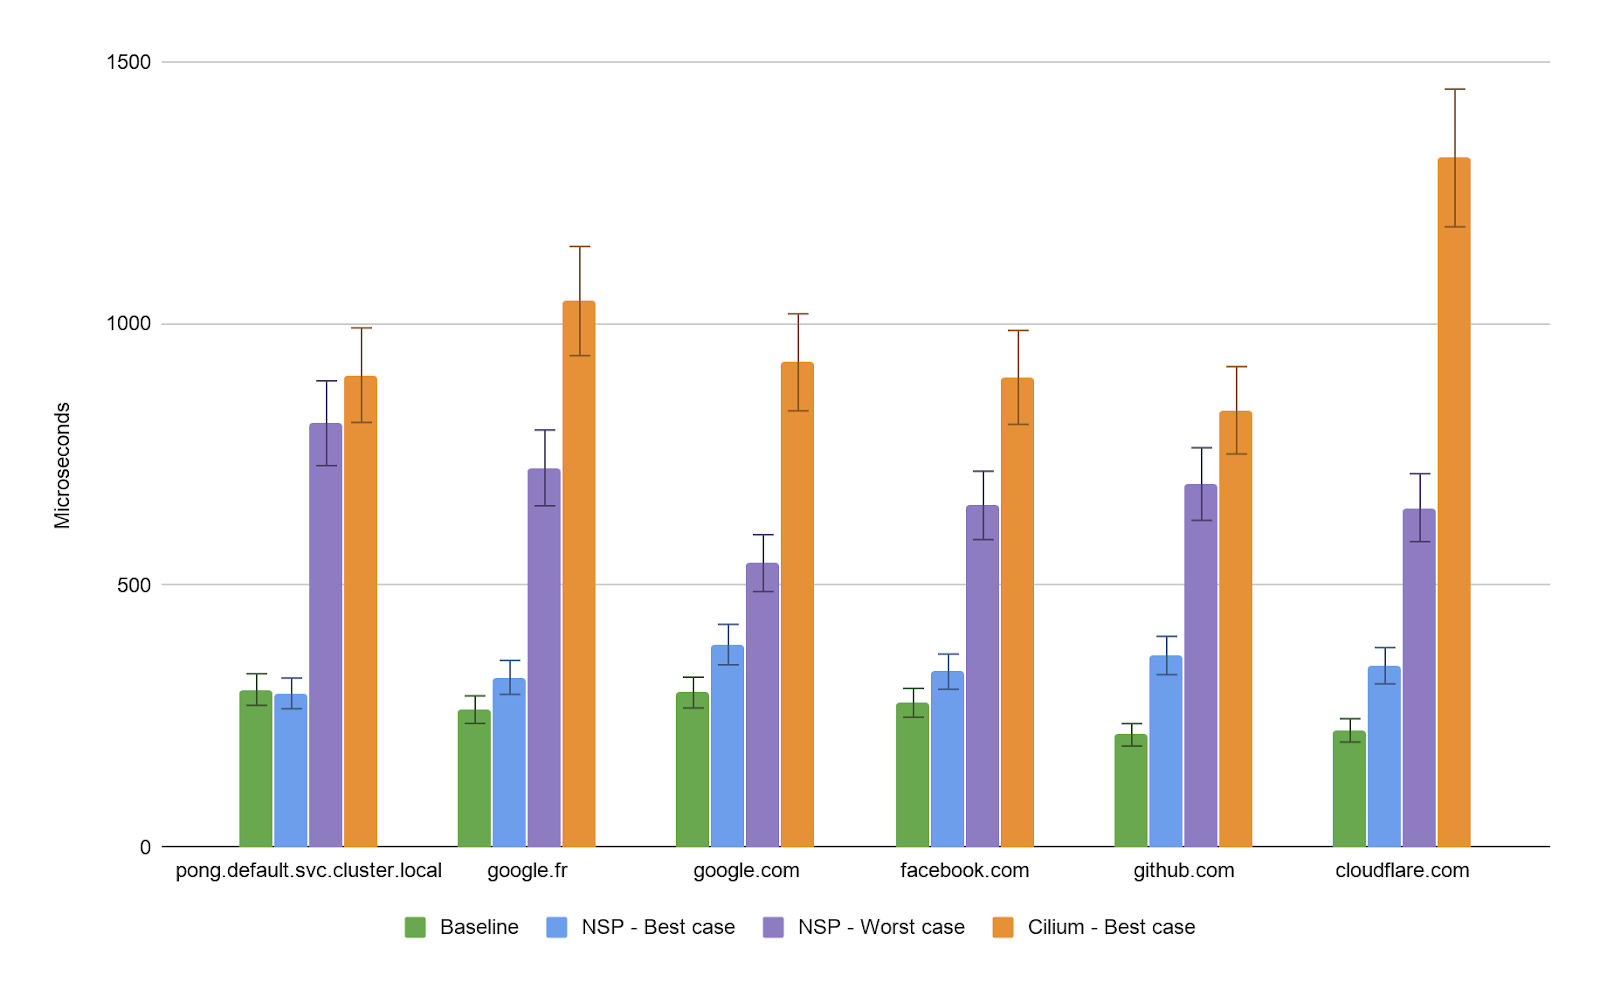
\includegraphics[width=\textwidth]{ProcessLevelNetworkSecurityMonitoring/img/round-trip-time.png}
  \caption*{Average round trip time per domain (averaged over 5000 A record queries per domain). The test was performed on a Linux ubuntu-bionic 4.15.0-88-generic, 2 vCPUs, 8 Gb RAM.}
  \label{fig:ProcessLevelNetworkSecurityMonitoring:round_trip_time}
\end{figure}

The best case scenario represents a situation where the tool was given the domain name, and therefore simply had to grant access without pushing any alerts back to user-space. The worst case scenario represents a situation where the tool had to alert on a request, thus triggering one of the kernel-space to user-space communication mechanisms available with eBPF. On the chart, NSP stands for Network Security Probe (the name of our tool).

\begin{figure}[h]
  \centering
  \includegraphics[width=\textwidth]{ProcessLevelNetworkSecurityMonitoring/img/CPU-RAM.png}
  \caption*{CPU and RAM usage of the user-space program over time. The test was performed on a Linux ubuntu-bionic 4.15.0-88-generic, 2 vCPUs, 8 Gb RAM.}
  \label{fig:ProcessLevelNetworkSecurityMonitoring:CPU_RAM}
\end{figure}

Although more testing would definitely be required to accurately assess the overhead in a real word environment, those results seem to confirm that there are no red flags to mapping eBPF packets to processes and assessing each packet at runtime. The worst case overhead is around 400 microseconds which is about half of the overhead of Cilium. This seems to confirm that in-kernel DNS parsing is a good strategy performance wise (but keep in mind that our DNS support is only partial for now, DNS parsing without loops is hard). Also, keep in mind that the 400 microseconds is the worst case scenario for the packets requiring the most processing. Our benchmark revealed that the actual overhead for a normal packet is closer to 200 microseconds for our tool and 250 microseconds for Cilium. Either way, those overheads are acceptable in a production environment.

\section{Conclusion}

There is still some work to be done before being able to consider this solution production ready. However this paper shows that it is possible to implement network monitoring \& enforcement at the process level with eBPF. Moreover, our design has the advantage that it is not intrusive in a Kubernetes setup, which means that it can be deployed fairly easily.

This paper also shows how excitingly easy it is to build complex security tools leveraging the insight that eBPF can provide into the depths of the kernel. Any new eBPF program type added to the kernel tree is an opportunity to generate new runtime security signals, that could be processed to provide new alerting and threats detection capabilities. That being said, the portability of such tools accross multiple kernel versions is still a work in progress~\cite{ProcessLevelNetworkSecurityMonitoring:CORE}.

As for this project, an exciting eBPF program type hasn’t been explored yet: \url{BPF_PROG_TYPE_CGROUP_SOCK}. This type of eBPF programs provides the opportunity to execute code when a process in a cgroup opens a network socket. It could be a good place to block attackers from opening RAW sockets, which is needed for various network attacks.

\bibliography{ProcessLevelNetworkSecurityMonitoring/biblio}
\nocite{*}
